\begin{center}
\Huge
Differentialligninger og grafer
\end{center}


\section*{Grafer}
\stepcounter{section}
Vi har indtil videre arbejdet primært med følgende klasser af 
differentialligninger.
\begin{align*}
	y' &= ky,\\
	y' &= b-ay, \textnormal{ og }\\
	y' &= ay(M - y)
\end{align*}

Vi kan se disse tre differentialligninger tegnet med $y$ langs førsteaksen og $y'$ langs andenaksen på Figur \ref{fig:diffs}
\begin{figure}[H]
	\centering
	\resizebox{0.45\textwidth}{!}
	{
	\begin{tikzpicture}
		\begin{axis}
			[axis lines = middle, 
			xmin = -1, xmax = 5,
			ymin = -1, ymax = 5,
			ticks = none, 
			xlabel = {$y$}, ylabel = {$y'$}
			]
			\addplot[thick, color = SeaGreen, domain = 0:5] {x};
			\draw[thick, dashed, color = Melon]	(axis cs: 3,2) -- (axis cs: 2,2) node[anchor = north, pos = 0.5] {1};
			\draw[thick, dashed, color = Melon]	(axis cs: 3,2) -- (axis cs: 3,3) node[anchor = west, pos = 0.5] {$k$};	
		\end{axis}
	\end{tikzpicture}
	}
	\resizebox{0.45\textwidth}{!}
	{
	\begin{tikzpicture}
		\begin{axis}
			[axis lines = middle, 
			xmin = -1, xmax = 5,
			ymin = -1, ymax = 5,
			ticks = none, 
			xlabel = {$y$}, ylabel = {$y'$}
			]
			\addplot[thick, color = SeaGreen, domain = 0:4] {4 - x};
			\draw[color = Melon, thick] (axis cs: -0.1, 4) -- (axis cs: 0, 4) node[pos = 0, anchor = east] {$b$};
			\draw[color = Melon, thick, dashed] (axis cs: 2,3) -- (axis cs: 1,3) node[pos = 0.5, anchor = south] {$1$};
			\draw[color = Melon, thick, dashed] (axis cs: 2,3) -- (axis cs: 2,2) node[pos = 0.5, anchor = west] {$a$};  			
		\end{axis}
	\end{tikzpicture}
	}
	\resizebox{0.45\textwidth}{!}
	{
	\begin{tikzpicture}
		\begin{axis}
			[axis lines = middle, 
			xmin = -1, xmax = 5,
			ymin = -1, ymax = 5,
			ticks = none, 
			xlabel = {$y$}, ylabel = {$y'$}
			]
			\addplot[thick, color = SeaGreen, domain = 0:4] {x*(4-x)};
			\draw[color = Melon, thick, dashed] (axis cs: 2, 4) -- (axis cs: 2,0) node[pos = 1, anchor = north] {$\frac{M}{2}$};			
		\end{axis}
	\end{tikzpicture}
	}
	\caption{Differentialligningerne $y'=ky$, $y' = b-ay$ og $y' = ay(M - y)$ henholdsvist.}
	\label{fig:diffs}
\end{figure}
\newpage
\begin{exa}
	En differentialligning er repræsenteret grafisk ved
	\begin{center}
		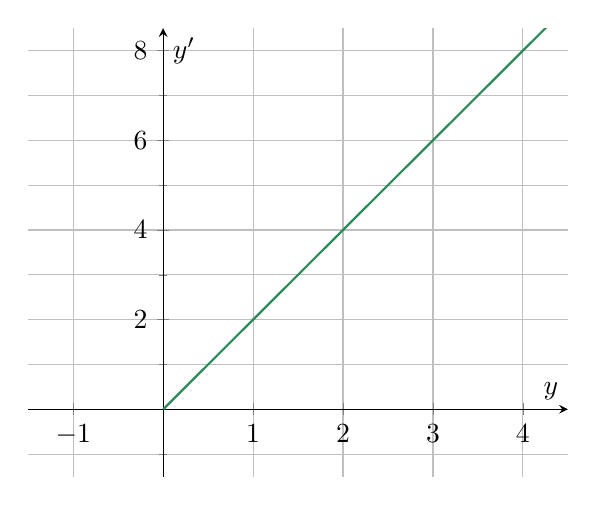
\begin{tikzpicture}
		\begin{axis}
			[axis lines = middle, 
			xmin = -1.5, xmax = 4.5,
			ymin = -1.5, ymax = 8.5,
			xlabel = {$y$}, ylabel = {$y'$},
			grid = both,
			minor y tick num = 1,
			]
			\addplot[thick, color = SeaGreen, domain = 0:4.5] {2*x};			
		\end{axis}
		\end{tikzpicture}
	\end{center}
	Af grafen kan vi se, at differentialligningen lyder
	\begin{align*}
		y' = 2y,
	\end{align*}
	og derfor har differentialligningen den fuldstændige løsning
	\begin{align*}
		y(x) = ce^{2x}.
	\end{align*}
\end{exa}


\begin{exa}
	Vi har følgende grafiske repræsentation for en differentialligning.
	\begin{center}
		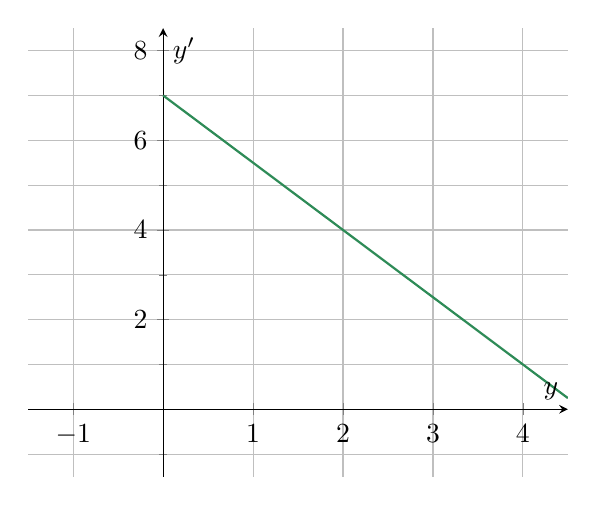
\begin{tikzpicture}
		\begin{axis}
			[axis lines = middle, 
			xmin = -1.5, xmax = 4.5,
			ymin = -1.5, ymax = 8.5,
			xlabel = {$y$}, ylabel = {$y'$},
			grid = both, 
			minor y tick num = 1, 
			]
			\addplot[thick, color = SeaGreen, domain = 0:4.5] {7-1.5*x};			
		\end{axis}
		\end{tikzpicture}
	\end{center}
	Af grafen kan vi se, at differentialligningen lyder
	\begin{align*}
		y' = 7-\frac{3}{2}y,
	\end{align*}
	og derfor har differentialligningen den fuldstændige løsning
	\begin{align*}
		y(x) = \frac{14}{3} + ce^{-\frac{3}{2}x}.
	\end{align*}
\end{exa}
Af Figur \ref{fig:diffs} kan vi se, at $y' = ay(M - y)$ har toppunkt, når $y = \frac{M}{2}$. Dette opskrives som en sætning og bevises. 
\begin{setn}
	Den logistiske differentialligning 
	\begin{align*}
		y' = ay(M-y)
	\end{align*}
	har maksimal vækst, når $y = \frac{M}{2}$. 
\end{setn}
\begin{proof}
	For at finde toppunktet, differentierer vi polynomiet 
	\begin{align*}
		p(y) =ay(M-y) = aMy-ay^2.
	\end{align*}
	Dette giver
	\begin{align*}
		p'(y) = aM-2ay
	\end{align*}
	Vi sætter dette lig 0 for at finde toppunktet.
	\begin{align*}
		aM-2ay = 0 \ &\Leftrightarrow \ aM = 2ay \\
		&\Leftrightarrow	 \ \frac{aM}{2a} = y \\
		&\Leftrightarrow	 \ \frac{M}{2} = y.
	\end{align*}
\end{proof}

\begin{exa}
	Vi betragter den logistiske differentialligning repræsenteret på Fig. \ref{fig:logist2}.
	\begin{figure}[H]
		\centering
		\begin{tikzpicture}
			\begin{axis}
				[
				axis lines = center, 
				xmin = -1, xmax = 5,
				ymin = -1, ymax = 3,
				xlabel = $y$, ylabel = $y'$, 
				]
				\draw[color = Melon, thick, dashed] (axis cs:0,2) to (axis cs: 2,2);
				\draw[color = Melon, thick, dashed] (axis cs:2,0) to (axis cs: 2,2);
				\addplot[thick, color = SeaGreen, domain = 0:4, samples = 200] {0.5*x*(4-x)};
			\end{axis}
		\end{tikzpicture}
		\caption{Grafisk repræsentation af en logistisk differentialligning.}
		\label{fig:logist2}
	\end{figure}
	Vi kan se, at denne parabel har rødder i 0 og 4. Derfor er differentialligningen på formen
	\begin{align*}
		y' = ay(4-y),
	\end{align*}
	og $M =4$. Vi bestemmer nu toppunktet af parablen.
	\begin{align*}
		a\frac{M}{2}(4-\frac{M}{2}) = a\frac{4}{2}(4-\frac{4}{2}) = a\cdot 2\cdot 2. = 4a
	\end{align*}
	Vi kan af Figur \ref{fig:logist2} se, at den maksimale vækst er $y' = 2$, så vi må have, at $4a = 2$, og $a=0.5$.
	Vores differentialligning lyder da
	\begin{align*}
		y' = 0.5y(4-y).
	\end{align*}
	Denne differentialligning har den fuldstændige løsning
	\begin{align*}
		y(x) = \frac{4}{1+ce^{-2x}}.
	\end{align*}
\end{exa}

\subsection*{Opgave 1}
Bestem fuldstændige løsninger til følgende grafisk repræsenterede differentialligninger
\begin{center}
	\resizebox{0.45\textwidth}{!}
	{
		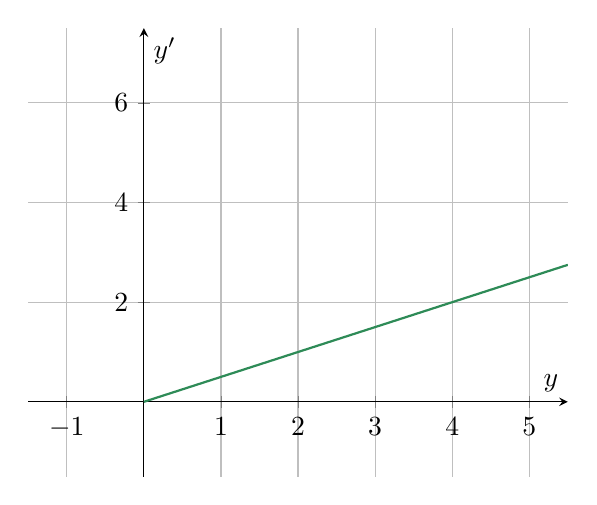
\begin{tikzpicture}
		\begin{axis}
			[axis lines = middle, 
			xmin = -1.5, xmax = 5.5,
			ymin = -1.5, ymax = 7.5,
			xlabel = {$y$}, ylabel = {$y'$},
			grid
			]
			\addplot[thick, color = SeaGreen, domain = 0:5.5] {0.5*x};			
		\end{axis}
		\end{tikzpicture}
	}
	\resizebox{0.45\textwidth}{!}
	{
		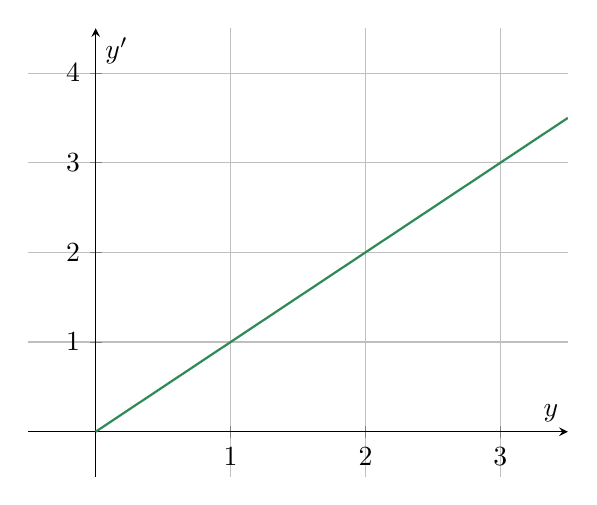
\begin{tikzpicture}
		\begin{axis}
			[axis lines = middle, 
			xmin = -0.5, xmax = 3.5,
			ymin = -0.5, ymax = 4.5,
			xlabel = {$y$}, ylabel = {$y'$},
			grid
			]
			\addplot[thick, color = SeaGreen, domain = 0:3.5] {x};			
		\end{axis}
		\end{tikzpicture}
	}
	\resizebox{0.45\textwidth}{!}
	{
		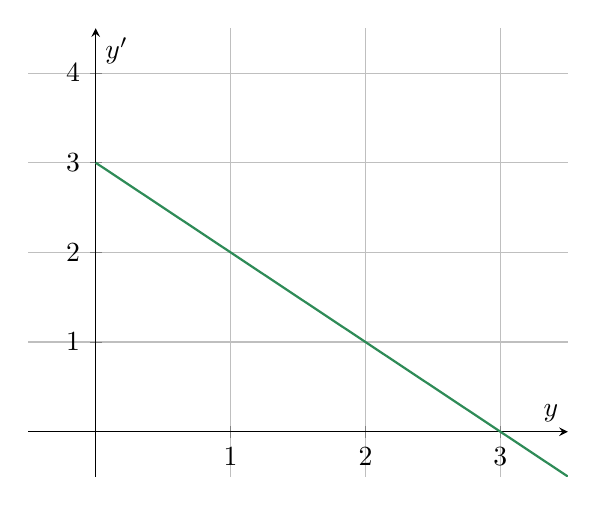
\begin{tikzpicture}
		\begin{axis}
			[axis lines = middle, 
			xmin = -0.5, xmax = 3.5,
			ymin = -0.5, ymax = 4.5,
			xlabel = {$y$}, ylabel = {$y'$},
			grid
			]
			\addplot[thick, color = SeaGreen, domain = 0:3.5] {3-x};			
		\end{axis}
		\end{tikzpicture}
	}
	\resizebox{0.45\textwidth}{!}
	{
		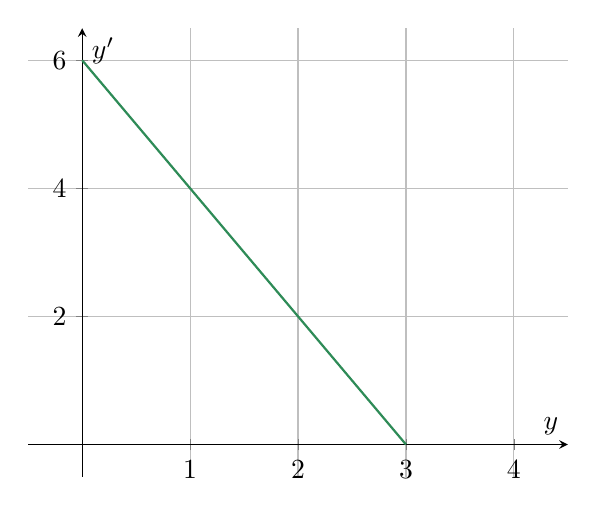
\begin{tikzpicture}
		\begin{axis}
			[axis lines = middle, 
			xmin = -0.5, xmax = 4.5,
			ymin = -0.5, ymax = 6.5,
			xlabel = {$y$}, ylabel = {$y'$},
			grid
			]
			\addplot[thick, color = SeaGreen, domain = 0:3] {6-2*x};			
		\end{axis}
		\end{tikzpicture}
	}
	\resizebox{0.45\textwidth}{!}
	{
		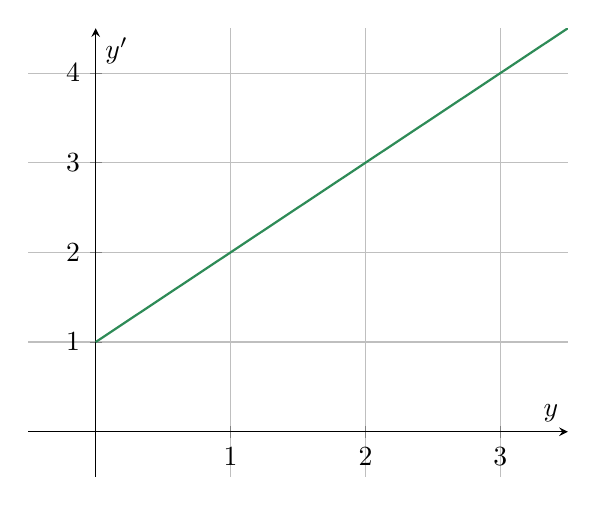
\begin{tikzpicture}
		\begin{axis}
			[axis lines = middle, 
			xmin = -0.5, xmax = 3.5,
			ymin = -0.5, ymax = 4.5,
			xlabel = {$y$}, ylabel = {$y'$},
			grid
			]
			\addplot[thick, color = SeaGreen, domain = 0:3.5] {1+x};			
		\end{axis}
		\end{tikzpicture}
	}
	\resizebox{0.45\textwidth}{!}
	{
		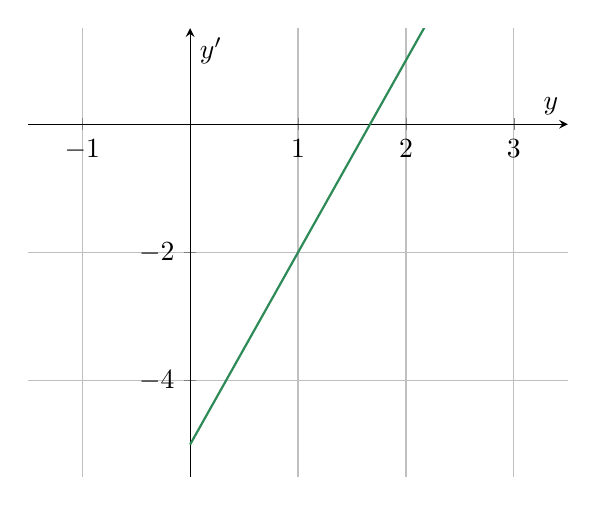
\begin{tikzpicture}
		\begin{axis}
			[axis lines = middle, 
			xmin = -1.5, xmax = 3.5,
			ymin = -5.5, ymax = 1.5,
			xlabel = {$y$}, ylabel = {$y'$},
			grid
			]
			\addplot[thick, color = SeaGreen, domain = 0:3.5] {-5+3*x};			
		\end{axis}
		\end{tikzpicture}
	}
	
\end{center}
\subsection*{Opgave 2}
Bestem fuldstændige løsninger til følgende grafisk repræsenterede differentialligninger.
\begin{center}
	\resizebox{0.45\textwidth}{!}
	{
		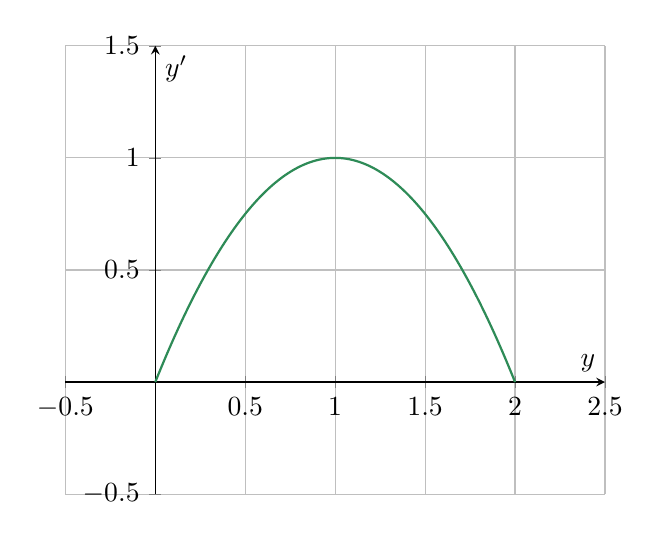
\begin{tikzpicture}
			\begin{axis}
				[
				axis lines = center, 
				xmin = -0.5, xmax = 2.5,
				ymin = -0.5, ymax = 1.5, 
				grid, 
				xlabel = $y$, ylabel = $y'$
				]
				\addplot[thick, color = SeaGreen, domain = 0:2, samples = 1000] {x*(2-x)};
			\end{axis}
		\end{tikzpicture}
	}
	\resizebox{0.45\textwidth}{!}
	{
		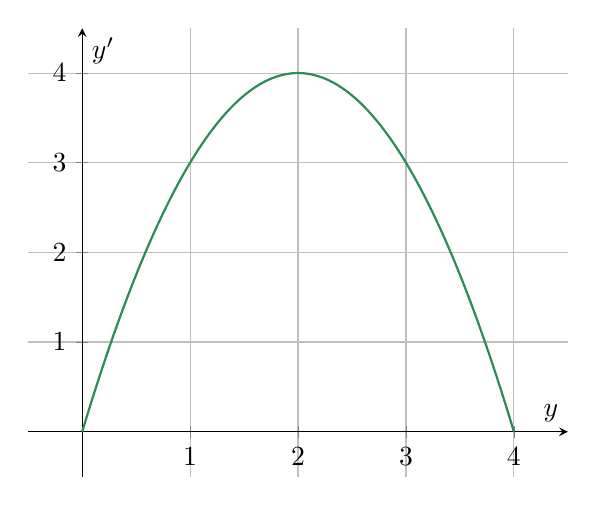
\begin{tikzpicture}
			\begin{axis}
				[
				axis lines = center, 
				xmin = -0.5, xmax = 4.5,
				ymin = -0.5, ymax = 4.5, 
				grid,
				xlabel = $y$, ylabel = $y'$
				]
				\addplot[thick, color = SeaGreen, domain = 0:4, samples = 1000] {x*(4-x)};
			\end{axis}
		\end{tikzpicture}
	}
	\resizebox{0.45\textwidth}{!}
	{
		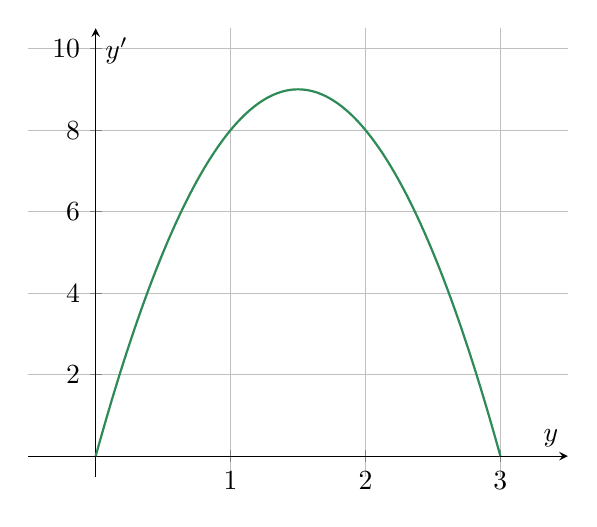
\begin{tikzpicture}
			\begin{axis}
				[
				axis lines = center, 
				xmin = -0.5, xmax = 3.5,
				ymin = -0.5, ymax = 10.5, 
				grid,
				xlabel = $y$, ylabel = $y'$
				]
				\addplot[thick, color = SeaGreen, domain = 0:3, samples = 1000] {4*x*(3-x)};
			\end{axis}
		\end{tikzpicture}
	}	
	\resizebox{0.45\textwidth}{!}
	{
		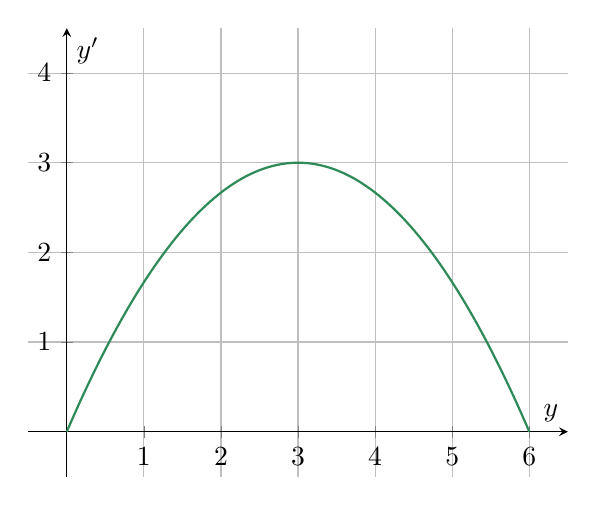
\begin{tikzpicture}
			\begin{axis}
				[
				axis lines = center, 
				xmin = -0.5, xmax = 6.5,
				ymin = -0.5, ymax = 4.5, 
				grid,
				xlabel = $y$, ylabel = $y'$
				]
				\addplot[thick, color = SeaGreen, domain = 0:6, samples = 1000] {(1/3)*x*(6-x)};
			\end{axis}
		\end{tikzpicture}
	}	
\end{center}
\newpage
\subsection*{Opgave 3}
\begin{enumerate}[label=\roman*)]
	\item Bestem en fuldstændig løsning til følgende grafisk repræsenterede differentialligning.
	\begin{center}
		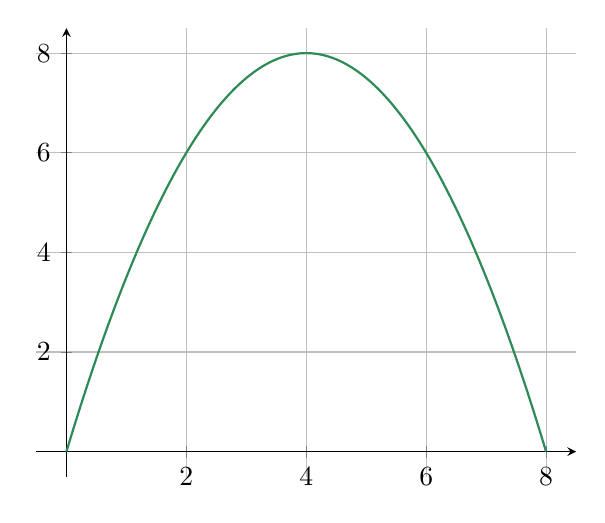
\begin{tikzpicture}
			\begin{axis}
				[
				axis lines = center, 
				xmin = -0.5, xmax = 8.5,
				ymin = -0.5, ymax = 8.5, 
				grid
				]
				\addplot[thick, color = SeaGreen, domain = 0:8, samples = 1000] {0.5*x*(8-x)};
			\end{axis}
		\end{tikzpicture}
	\end{center}
	\item Bestem nu en partikulær løsning, der går gennem punktet $(0,4)$. 
	\item Hvad er væksten af $y$, når $y=5$?
	\item Bestem $y(2)$. 
\end{enumerate}
\newpage
\subsection*{Opgave 4}
\begin{enumerate}[label=\roman*)]
	\item Bestem den partikulære løsning til differentialligningen repræsenteret på følgende graf, der opfylder, at den går gennem punktet $(0,7)$.
	\begin{center}
		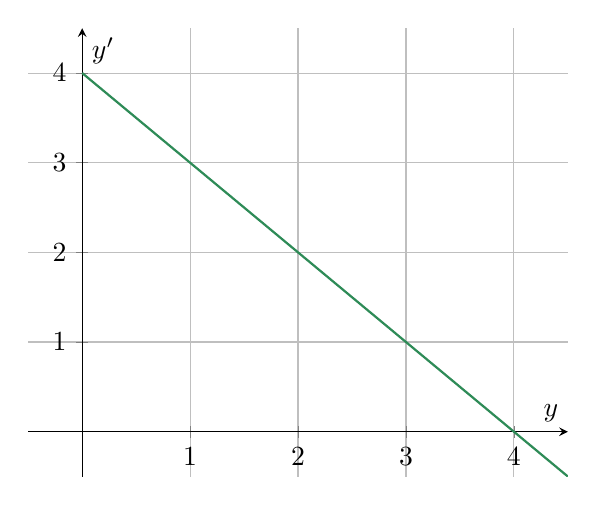
\begin{tikzpicture}
		\begin{axis}
			[axis lines = middle, 
			xmin = -0.5, xmax = 4.5,
			ymin = -0.5, ymax = 4.5,
			xlabel = {$y$}, ylabel = {$y'$},
			grid
			]
			\addplot[thick, color = SeaGreen, domain = 0:4.5] {4-x};			
		\end{axis}
		\end{tikzpicture}
	\end{center}
	\item Bestem en partikulær løsning til differentialligningen repræsenteret på følgende graf, der går gennem punktet 
	$(0,\sqrt{2})$.
	\begin{center}
		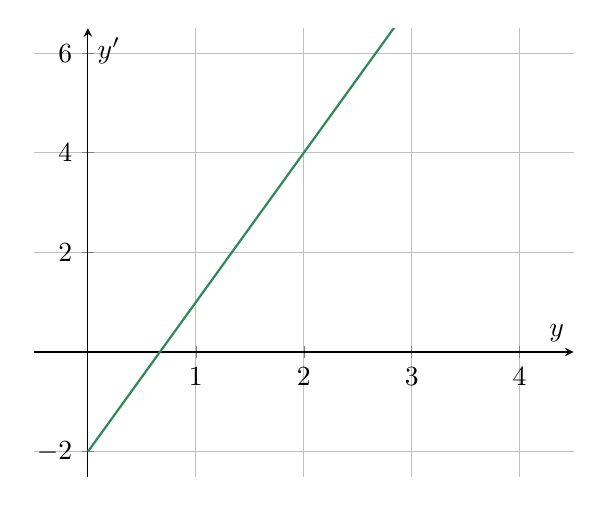
\begin{tikzpicture}
		\begin{axis}
			[axis lines = middle, 
			xmin = -0.5, xmax = 4.5,
			ymin = -2.5, ymax = 6.5,
			xlabel = {$y$}, ylabel = {$y'$},
			grid
			]
			\addplot[thick, color = SeaGreen, domain = 0:4.5] {-2+3*x};			
		\end{axis}
		\end{tikzpicture}
	\end{center}
\end{enumerate}

\newpage 

\subsection*{Opgave 5}
\begin{enumerate}[label=\roman*)]
	\item Bestem en fuldstændig løsning til følgende grafisk repræsenterede differentialligning.
	\begin{center}
		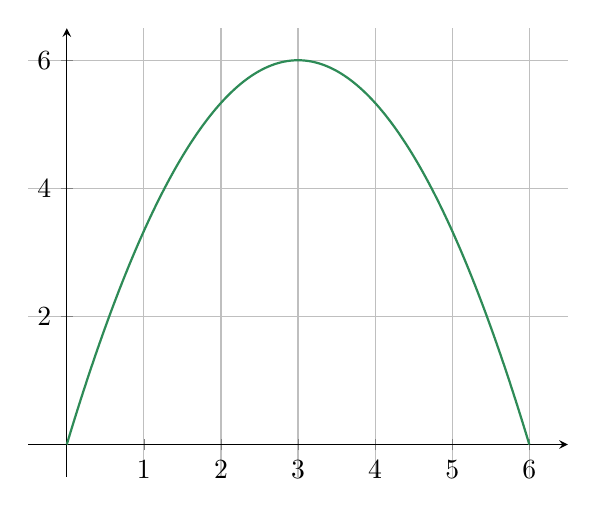
\begin{tikzpicture}
			\begin{axis}
				[
				axis lines = center, 
				xmin = -0.5, xmax =6.5 ,
				ymin = -0.5, ymax = 6.5, 
				grid
				]
				\addplot[thick, color = SeaGreen, domain = 0:6, samples = 1000] {(2/3)*x*(6-x)};
			\end{axis}
		\end{tikzpicture}
	\end{center}
	\item Bestem nu en partikulær løsning, der går gennem punktet $(0,12)$.
	\item Hvad er væksten af $y$, når $y=2$?
	\item Bestem $y(4)$.  
\end{enumerate}
\subsection*{Opgave 6}
\begin{enumerate}[label=\roman*)]
	\item En ret linje $y' = b-ay$ går gennem punkterne $(1,3)$ og $(3,9)$. Bestem den fuldstændige løsning $y$ til den
	differentialligning, der er repræsenteret ved denne rette linje.
	\item En ret linje $y' = b-ay$ går gennem punkterne $(1,2)$ og $(2,4)$. Bestem den partikulære løsning $y$ til den 
	differentialligning, der er repræsenteret ved denne rette linje.
\end{enumerate}

\subsection*{Opgave 7}
\begin{enumerate}[label=\roman*)]
	\item Følgende sammenhæng mellem $y$ og $y'$ er givet.
	\begin{center}
	\begin{tabular}{c|c|c|c|c|c|c}
		$y$ & 1.3 & 3.2 & 5.7 & 6.9 & 10.68 & 11.97\\
		\hline
		 $y'$ & 69.5 & 58.1 & 42.4 & 44.7 & 18.4 & 28.35
	\end{tabular}
	\end{center}
	Det antages, at sammenhængen mellem $y$ og $y'$ er givet ved
	\begin{align*}
		y' = b-ay.
	\end{align*}
	Brug datasættet til at bestemme den fuldstændige løsning $y$. 
\end{enumerate}

\newpage

\subsection*{Opgave 8}
	Et objekt med en temperatur på $100^\circ$C stilles i et lokale med en temperatur på $19^\circ$C. Det er oplagt, at temperaturen falder langsomme og langsommere jo nærmere
	temperaturen kommer på den omkringliggende temperatur. Vi antager, at temperaturfaldets hastighed er proportional med objektets temperatur eller mere præcist, at 
	temperaturen og temperaturfaldet opfylder differentialligningen
	\begin{align*}
		y' = -k(y-19) = -ky+19k.
	\end{align*}
	\begin{enumerate}[label=\roman*)]
		\item Bestem den fuldstændige løsning til differentialligningen. 
		\item Udnyt, at $y(0) = 100$ til at bestemme konstanten $c$. 
		\item Udnyt, at temperaturen efter 5 minutter er $80^\circ$C til at bestemme $k$. 
		\item Opskriv modellen $y(t)$ for temperaturen af objektet. 
	\end{enumerate}
